\documentclass[12pt]{report}
\usepackage{amsmath, amssymb, amsthm}
\usepackage{graphicx}
\usepackage{hyperref}
\usepackage[utf8]{inputenc}
\usepackage[margin=1in]{geometry}
\usepackage{float}
\usepackage{titlesec}
\usepackage{caption}
\usepackage{enumitem}
\usepackage{bm}
\usepackage{physics}
\usepackage{mathrsfs}
\usepackage{float}

\titleformat{\chapter}{\Huge\bfseries}{\thechapter}{16pt}{\Huge\bfseries}
\titleformat{\section}{\Large\bfseries}{\thesection}{1em}{}
\titleformat{\subsection}{\large\bfseries}{\thesubsection}{1em}{}
\titleformat{\subsubsection}{\bfseries}{\thesubsubsection}{1em}{}

\newtheorem{theorem}{Theorem}[section]
\newtheorem{definition}[theorem]{Definition}
\newtheorem{example}[theorem]{Example}
\newtheorem{remark}[theorem]{Remark}

\title{Functional Analysis in Brownian Motion: A Comprehensive Framework}
\author{Aash Makwana \\ Instructor: Dr. Tracey Balehowsky \\ \\ 
MATH 617 - Functional Analysis \\ \\ University of Calgary}
\date{April 14, 2025}

\begin{document}

\maketitle

\begin{abstract}
\textit{Brownian motion $B_t$, a continuous-time stochastic process; Functional analysis, foundation for infinite dimensional spaces. In this project, we use functional-analytic tools to study Brownian motion, focusing on the proof for existence of Brownian motion\cite{bobrowski} originally given by Wiener. Using Hilbert space techniques, we reconstruct Wiener's proof within the framework of \textit{abstract Wiener space} $(H, \mathcal{B}, \mu)$, where $H$ is a Hilbert space, $\mathcal{B}$ is the Borel $\sigma$-algebra, and $\mu$ is Wiener measure. We further try to examine the \textit{Cameron–Martin theorem}\cite{karatzas}, which describes how Wiener measure transforms under translations by elements of the \textit{Cameron–Martin space} $H$, formally stating that for any $h \in H$, the Radon–Nikodym derivative satisfies  
    \[
        \frac{d\mu_h}{d\mu}(x) = \exp \left( \langle h, x \rangle_H - \frac{1}{2} \| h \|_H^2 \right).
    \]
    Additionally, we will try to understand the \textit{Kosambi–Karhunen–Lo\`eve theorem}\cite{karatzas}, which provides a spectral decomposition of stochastic processes, expressing $B_t$ as an infinite sum of orthogonal functions $\{\phi_n\}$ with uncorrelated coefficients:
    \[
        B_t = \sum_{n=1}^{\infty} Z_n \phi_n(t),
    \]
    where $\{Z_n\}$ are uncorrelated random variables. These results highlight the interplay between measure theory, Hilbert spaces, and stochastic processes, offering a functional-analytic perspective on Brownian motion.}
\end{abstract}

\tableofcontents

\chapter{Introduction}
\section{Objective and Motivation}
The objective of our project is to establish a functional analysis foundation for Brownian motion, which serves as a main part in the theory of modern stochastic processes. Our approach for this whole project is structured around three main topics that capture the essence of infinite-dimensional analysis in probability theory:

\begin{itemize} \item \textbf{Wiener’s Abstract Space Formulation:} Wiener's construction with use of abstract Wiener spaces provides a Hilbert space framework for modeling Brownian paths. It also formalizes the notion of Gaussian measures in infinite dimensions; 
\item \textbf{Cameron–Martin Measure Transformations:} Measure transformations under the Cameron-Martin theorem which characterizes the quasi-invariance of Wiener measure under shifts by elements of the Cameron-Martin space and thus plays a fundamental role in stochastic calculus and large deviations theory;
\item \textbf{Karhunen–Loève Spectral Analysis:} Spectral decomposition via the Karhunen-Loeve theorem which gives an orthogonal expansion of Brownian motion in terms of eigenfunctions of its covariance operator thus allowing for dimensionality reduction and efficient representations. \end{itemize}

Together, these tools form a necessary toolkit for the infinite-dimensional stochastic systems development. We will also provide \textit{Python} code for certain examples which we have used in each section to describe the topic. From there, foundations apply to an integral function in a vast assortment of applications that range from quantitative finance, through statistical physics and signal processing, to modern machine learning where the behavior of intricate random phenomena in settings that are high-dimensional or function spaces is of paramount significance.

\section{Broader Context and Historical Development}

Brownian motion was originally introduced as a physical phenomenon which was first observed in pollen particles suspended in water. This created a mathematical foundation in the early 20\textsuperscript{th} century, startinf with research works of Norbert Wiener and Paul Lévy. 
The first continuous-time stochastic process with continuous sample paths was developed by Wiener in 1923 which further developed the \textit{Wiener measure}, a probability measure on the space of continuous functions.

The study and research in Brownian motion lies at the intersection of several tools of mathematics,:
\begin{itemize}
    \item \textbf{Probability Theory and Stochastic Processes}: Brownian motion forms the basis of Itô calculus, martingale theory, and diffusion processes. It act as a canonical model for continuous-time random motion.
    \item \textbf{Measure Theory and Abstract Integration}: Use of Gaussian measures on infinite-dimensional spaces and Radon–Nikodym derivatives.
    \item \textbf{Functional Analysis}: It uses tools like Hilbert and Banach space structures, operator theory, and infinite-dimensional integration.
    \item \textbf{Spectral Theory and Harmonic Analysis}: Used in the Karhunen–Loève expansion and eigenfunction decompositions of covariance operators.
\end{itemize}

\textbf{Abstract Wiener spaces} were first time introduced by Leonard Gross in the 1960s. The main foundation was to formalize the embedding of a Hilbert space into a Banach space for defining Gaussian measures in infinite dimensions. After that the formulation of the \textbf{Cameron–Martin theorem} in 1945 was addressed as the fundamental question of how Wiener measure behaves under translation by deterministic functions. This created a much deeper understanding of the quasi-invariance of measures. 

\medskip

\noindent\textbf{Open Questions and Modern Directions.} Today, the field of Brownian motion continues to evolve which have active research, some of them areL
\begin{itemize}
    \item Development of robust theories for non-Gaussian processes (e.g., fractional Brownian motion or Lévy processes) in infinite dimensions;
    \item Deepening the theory of stochastic partial differential equations (SPDEs), where Brownian motion acts as the driving noise in infinite-dimensional systems;
    \item Functional analytic foundations for path space analysis in quantum mechanics and machine learning, especially via reproducing kernel Hilbert spaces (RKHS).
\end{itemize}

The questions that initiated this line of research and remain central to contemporary research in probability, statistics, and functional analysis.



\chapter{Foundations of Brownian Motion}
\section{Formal Definition}
\begin{definition}[Standard Brownian Motion]
A standard Brownian motion (also called one-dimensional Wiener process) is a stochastic process \(\{W_t\}_{t \geq 0}\) on a probability space \((\Omega, \mathcal{F}, \mathbb{P})\) satisfies:
\begin{enumerate}
    \item \(W_0 = 0\) (almost surely),
    \item Continuous paths: \(t \mapsto W_t\) is continuous in t with \(\mathbb{P}\)-a.s.,
    \item Independent increments: \(W_{t} - W_s \sim \mathcal{N}(0, t-s)\) for \(t > s\),
    \item Stationary increments: Distribution of \(W_{t+h} - W_s\) depends only on \(h\).
\end{enumerate}
\end{definition}
\noindent
\textbf{Brownian motion $W(t)$ has the probability density function of}  $f_{W_{t}}(x) = \frac{1}{\sqrt{2 \pi t}}e^{\frac{-x^2}{2t}} $.\\
\\
\noindent
A standard $d-$dimensional Brownian motion is a vector-valued stochastic process
\[
W_t =  (W^{(1)}_t ,W^{(2)}_t ,..., W^{(d)}_t )
\]
where, $W^{(i)}_t$ are independent, standard one-dimensional Brownian motion. A Brownian motion with an initial value of $x$ is obtained by adding $x$ to a standard wiener. Independent increments refer to the concept that for every positive real number, there is a corresponding choice that does not affect the outcome. The sequence of non-negative real numbers $ 0, s_1, t_1, s_2, t_2,.., s_n, t_n,.., \infty,$ represents the random variables with increment values. The term stationary increments refers to the condition where for any values of $s$ and $t$ less than infinity, the increments are independent of each other. The distribution of the increment $W_t+s - W_s$ is the same as $W_t-W_0 = W_t$. In general, a stochastic process with stationary, independent increments is referred to as an L´evy process. 

\begin{figure}[H]
    \centering
    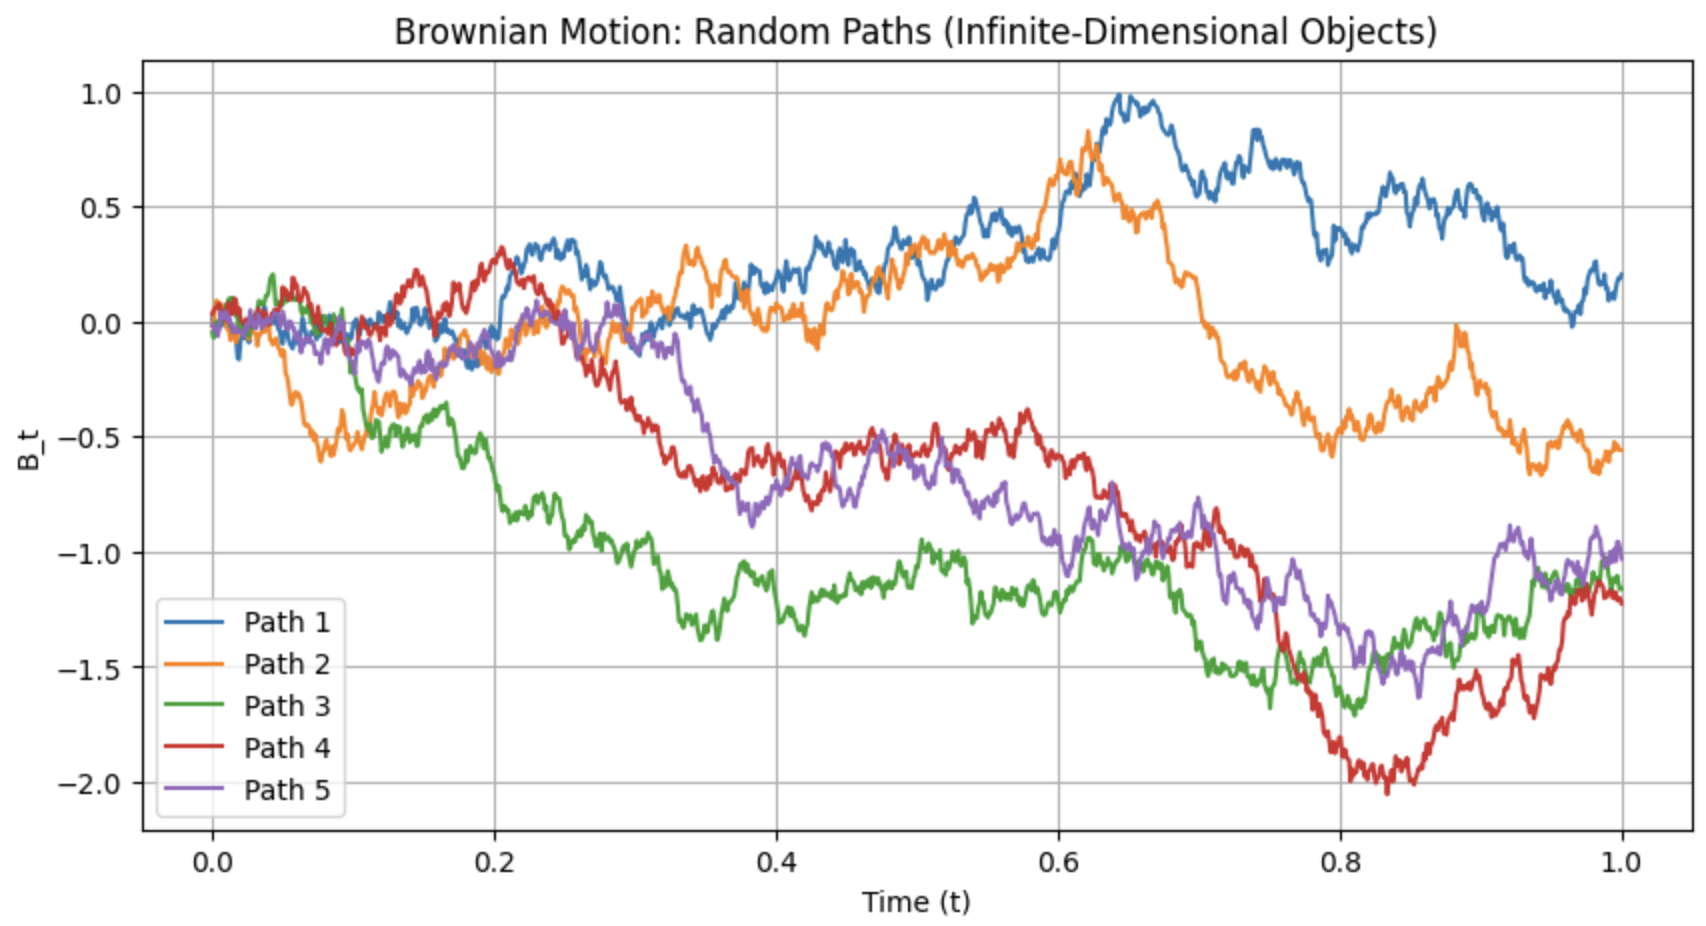
\includegraphics[width=0.84\linewidth]{Brownian Motion.png}
    \caption{Standard Brownian Motion, \textit{Code: A.1}}
    \label{fig:enter-label}
\end{figure}

\section{Random Walks}
In our further report, we will show Wiener's construction. Before that in this section we will try to explain a basic intuition of Brownian Motion using Random Walks.

\subsection{Symmetric Random Walk}
Creating a Symmetric Random Walk is ideal to repeatedly toss a
fair coin $(p= q = 1/2)$. Let $X_j$ be the random variable representing the outcome of the $j^{th}$ coin toss as:
\[
X_j = \begin{cases}
    1 & \text{outcome is head} \\
    -1& \text{outcome is tail}
\end{cases} \ \ \ j = 1,2,...
\]
Now defining the stochastic process $\{M_k\}_{k\geq 0}$ with initial condition $M_0 = 0$ and
\[
M_k = \sum_{j=1}^kM_j\ ,k= 1,2,...
\]
where $M_k$ is a Symmetry Random Walk.

\begin{figure}[H]
    \centering
    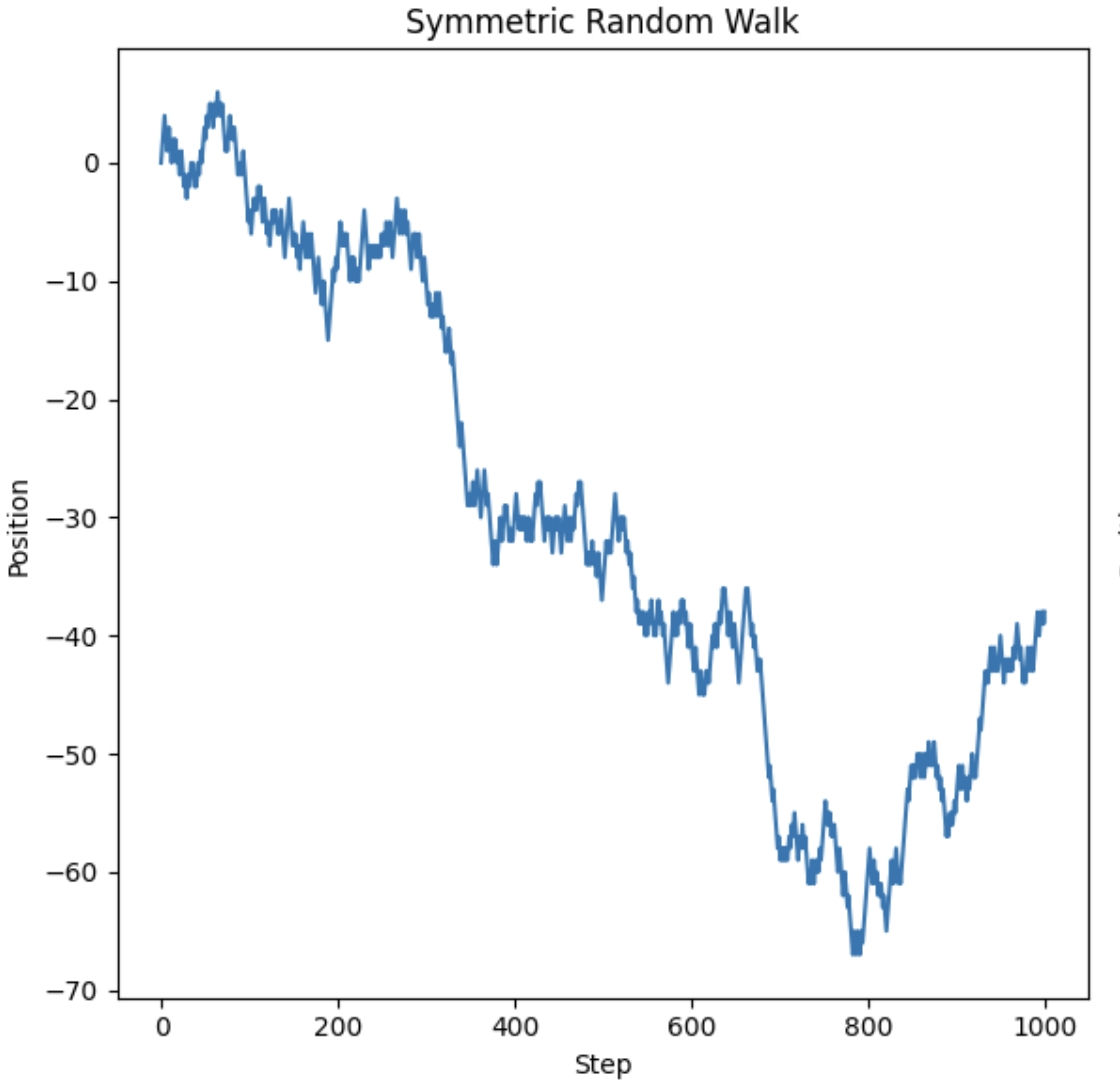
\includegraphics[width=0.65\linewidth]{Symmetric Random Walk.png}
    \caption{Symmetric Random Walk, Each step is either $+1$ or $-1$ with equal probability, The walk is generated by taking the cumulative sum of these steps, starting at $0$ with a variance that increases linearly with the number of steps. \textit{Code: A.2}}
    \label{fig:enter-label}
\end{figure}

\noindent
The increments of Symmetric Random Walk, $M_{k_{i+1}} - M_{k_{i}}$ has expected value $\mathbb{E}(M_{k_{i+1}} - M_{k_{i}}) = 0$ and variance $\text{Var}(M_{k_{i+1}} - M_{k_{i}}) = k_{i+1}-k_{i}$.

\subsection{Scaled Random Walk}
A Symmetric Random Walk does not help us much to create a Brownian motion. However we can elevate the same procedure by changing the rules of the coin toss, by speeding up time and scaling down the step size, hence creating a Scaled Random Walk.\\
\\
\noindent
Let us start by a fixed integer $n$, then we can define Scaled Random Walk using Symmetric Random Walk as:
\[
W^{(n)}(t) = \frac{1}{\sqrt{n}}M_{nt}
\]
for all $t\geq 0$ such that $nt$ is an integer.\\
\\
\noindent
The increments of Scaled Random Walk, $W^{(n)}(t) - W^{(n)}(s)$ has expected value $\mathbb{E}(W^{(n)}(t) - W^{(n)}(s)) = 0$ and variance $\text{Var}(W^{(n)}(t) - W^{(n)}(s)) = t-s$.

\begin{figure}[H]
    \centering
    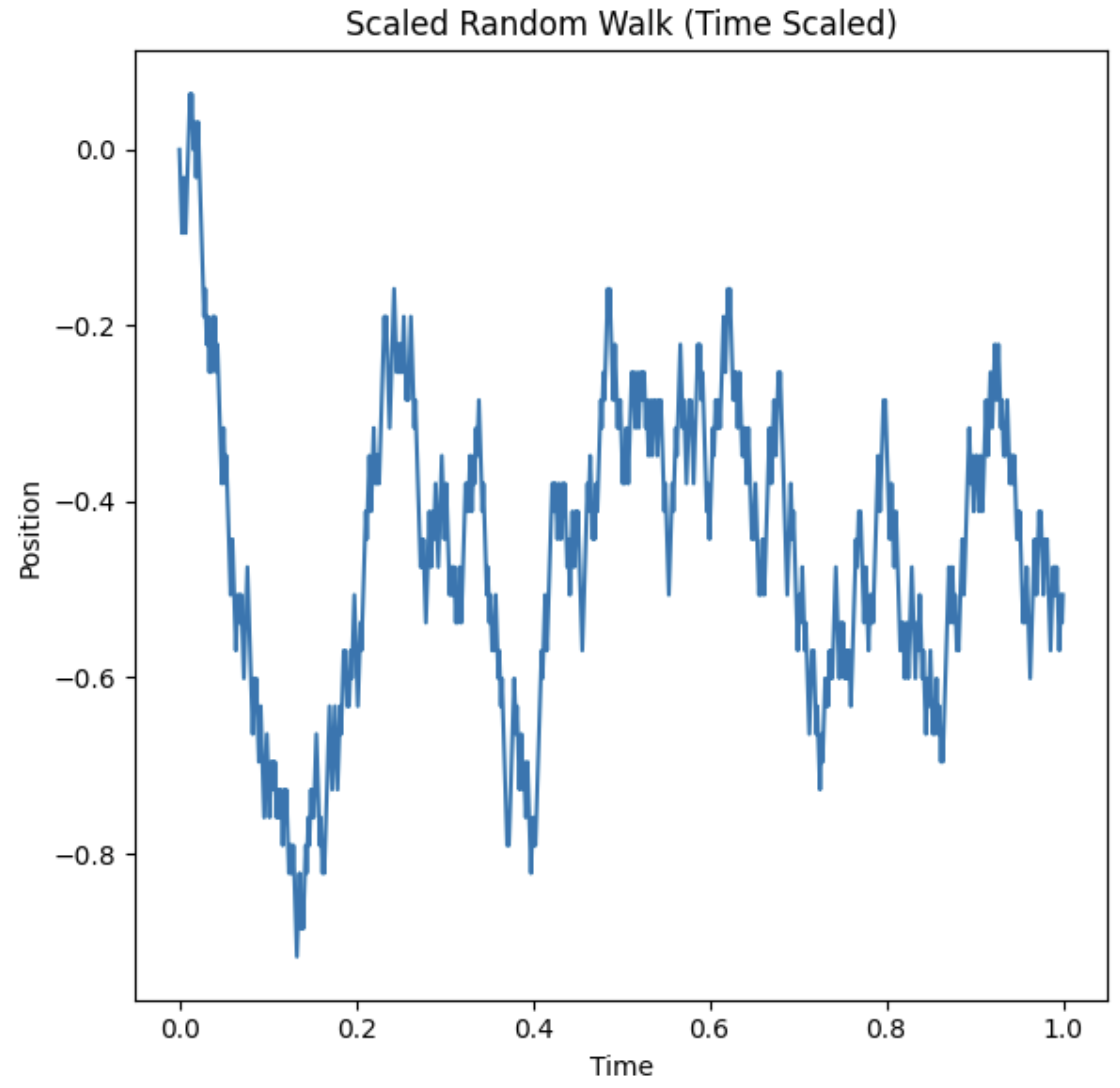
\includegraphics[width=0.65\linewidth]{Scaled Random Walk.png}
    \caption{Scaled Random Walk, this walk is generated over a time interval $[0, T]$, with each step's magnitude adjusted to maintain proper scaling, this scaling shows the properties of a Wiener process (Brownian motion), where variance grows linearly with time. \textit{Code: A.2}}
    \label{fig:enter-label}
\end{figure}

\section{Key Properties and Their Implications}
\subsection{Non-Differentiability}
As Brownian motion shows quadratic variation at rate one per unit time, it cannot be continuously differentiable. In fact, the paths of a Brownian motion are almost surely nowhere differentiable.
\begin{theorem}[Paley, Wiener and Zygmund 1933]
For almost every \(\omega \in \Omega\), the path \(t \mapsto W_t(\omega)\) is nowhere differentiable.
\end{theorem}

\subsection{Quadratic Variation}
\begin{definition}[Quadratic Variation]
The quadratic variation of \(W_t\) on \([0, T]\) is:
\[
\langle W \rangle_T = \lim_{\|\Pi\| \to 0} \sum_{i=1}^n (W_{t_i} - W_{t_{i-1}})^2 = T \quad \text{a.s.},
\]
where \(\Pi = \{0 = t_0 < t_1 < \cdots < t_n = T\}\).
\end{definition}

\begin{figure}[H]
    \centering
    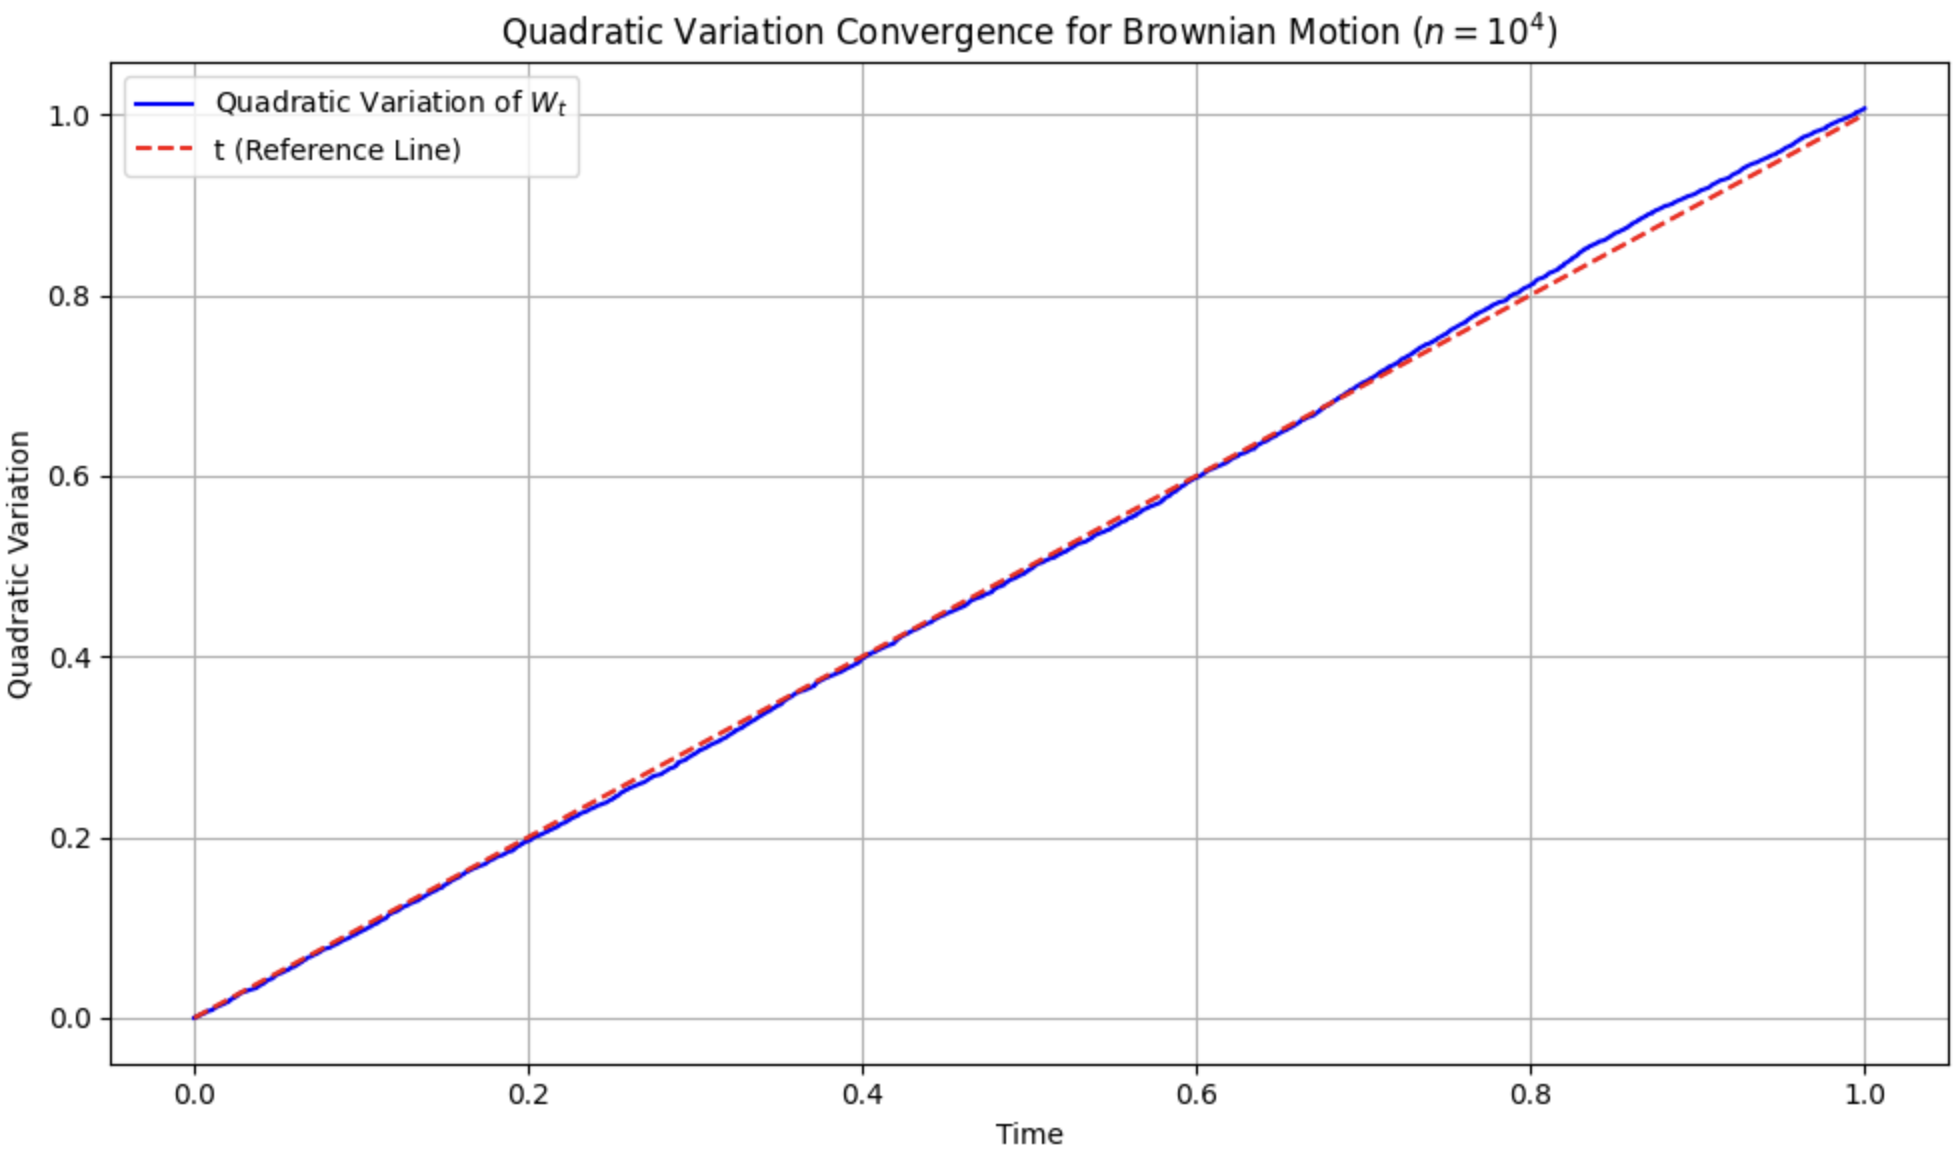
\includegraphics[width=0.75\textwidth]{Quadratic Convergence.png}
    \caption{Quadratic variation convergence for Brownian motion (simulated with \(n=10^4\) partitions). \textit{Code: A.3}}
    \label{fig:qv}
\end{figure}

\chapter{Wiener’s Construction}
\section{Measure-Theoretic Foundations}
\begin{definition}[Abstract Wiener Space]
A triple \((H, \mathcal{B}, \mu)\) where:
\begin{itemize}
    \item \(H\): Cameron-Martin space of absolutely continuous functions with \(f' \in L^2([0,1])\),
    \item \(\mathcal{B}\): Completion of \(H\) under the sup-norm \(\|f\|_\infty = \sup_{t \in [0,1]} |f(t)|)\),
    \item \(\mu\): Wiener measure, the unique Gaussian measure on \(\mathcal{B}\) with covariance \(\mathbb{E}[W_t W_s] = \min(t,s)\).
\end{itemize}
\end{definition}
\noindent
\textbf{Example:} (Cylinder Sets and Measure Consistency)
Cylinder sets serve as the foundational building blocks for constructing measures on infinite-dimensional function spaces. Explaining it specifically in Brownian motion, a \textbf{cylinder set} \(C \subset \mathcal{B}\) is defined by restricting paths to specific behaviors at finitely many times. Defining it explicitly, given times \(0 = t_0 < t_1 < \cdots < t_n \leq 1\) and a Borel set \(A \subset \mathbb{R}^n\), the cylinder set is:  
\[
C = \left\{ f \in \mathcal{B} \,:\, \big(f(t_1), f(t_2) - f(t_1), \ldots, f(t_n) - f(t_{n-1})\big) \in A \right\}.
\]
Here, the increments \(f(t_i) - f(t_{i-1})\) are restricted to be within \(A\). The Wiener measure \(\mu\) assigns probabilities to such sets by integrating the joint density of these increments, which are independent and normally distributed under Brownian motion. It can be stated for \(A \subset \mathbb{R}^n\) as,  
\[
\mu(C) = \int_A \prod_{i=1}^n \frac{1}{\sqrt{2\pi(t_i - t_{i-1})}} \exp\left(-\frac{(x_i - x_{i-1})^2}{2(t_i - t_{i-1})}\right) dx_1 \cdots dx_n,
\]  
where \(x_0 = 0\) by convention. Each term in the product corresponds to the transition density of Brownian motion between times \(t_{i-1}\) and \(t_i\), reflecting the Markov property: the increment \(W_{t_i} - W_{t_{i-1}}\) depends only on the elapsed time \(t_i - t_{i-1}\), not the prior path.

\section{Orthogonal Expansions and Fourier Series}

\subsection{Wiener’s Fourier Representation}

Fourier Basis Expansion: Let $\{\varphi_n(t)\}_{n \geq 1}$ denote the orthonormal sine basis on $[0,1]$:
\[
\varphi_n(t) = \sqrt{2} \sin\left( \frac{(2n - 1)\pi t}{2} \right), \quad n \geq 1.
\]
Then, Brownian motion $W_t$ admits the following series expansion:
\[
W_t = \sum_{n=1}^\infty Z_n \varphi_n(t), \quad Z_n \sim \mathcal{N}(0,1) \text{ i.i.d.}
\]

This expansion provides a concrete representation of Brownian paths as infinite-dimensional Gaussian series in the Hilbert space $L^2([0,1])$. It also connects with the Karhunen–Loève theorem as a special case for Brownian motion. We have described this portion in detail in Chapter 5.

\subsection{Convergence Analysis}

\begin{theorem}[Uniform Almost Sure Convergence]\label{thm:fourier_convergence}
Let $W_t = \sum_{n=1}^\infty Z_n \varphi_n(t)$ be the Fourier expansion of Brownian motion. Then the series converges uniformly on $[0,1]$ with probability one.
\end{theorem}

\begin{proof}[Sketch of Proof]
This result follows from the \textit{Itô–Nisio theorem}, which states that for a sequence of independent, symmetric random variables taking values in a separable Banach space (e.g., $C([0,1])$), almost sure convergence of partial sums follows from pointwise convergence and tightness. Since the basis functions $\varphi_n(t)$ are uniformly bounded and $Z_n \sim \mathcal{N}(0,1)$, the required conditions are satisfied, implying almost sure uniform convergence.
\end{proof}

This representation emphasizes the infinite-dimensional structure of Brownian paths, and convergence almost surely (rather than in mean square) reveals the deep probabilistic behavior of these random series in the path space.








\section{Wiener’s Stepwise Construction}
\subsection{Finite-Dimensional Approximations}

The method we will show here for constructing Brownian motion (Wiener's space) involves approximating it in finite-dimensional spaces using dyadic partitions. This construction makes easy the use of projective limits and establishes the existence of a probability measure on the path space.

\begin{itemize}
    \item \textbf{Dyadic Partitioning:}  
    Lets start by a \( n \in \mathbb{N} \), then partition the interval \([0,1]\) into \(2^n\) equal subintervals:
    \[
    t_k = \frac{k}{2^n}, \quad k = 0, 1, \dotsc, 2^n.
    \]
    Using this we'll define an approximation to Brownian motion by specifying its values on these dyadic points.

    \item \textbf{Gaussian Increments:}  
    Further, constructing a finite-dimensional distribution \(\mu_n\) on \(\mathbb{R}^{2^n}\) by assigning independent Gaussian increments to successive subintervals:
    \[
    W_{t_k} - W_{t_{k-1}} \sim \mathcal{N}(0, 2^{-n}) \quad \text{independently for } k = 1, \dotsc, 2^n.
    \]
    The random vector \( (W_{t_1}, W_{t_2}, \ldots, W_{t_{2^n}}) \) is then defined recursively by summing these increments.

    \item \textbf{Kolmogorov Consistency and Projective Limit:}  
    The family of measures \( \{\mu_n\}_{n \in \mathbb{N}} \) satisfies the Kolmogorov consistency conditions: for each \( n \), the marginal of \(\mu_{n+1}\) on \( \mathbb{R}^{2^n} \) coincides with \( \mu_n \). Thus, by Kolmogorov’s Extension Theorem, there exists a unique probability measure \( \mu \) on the infinite product space (e.g., \( \mathbb{R}^{\mathbb{N}} \) or a suitable function space such as \( C([0,1]) \)) such that the finite-dimensional distributions agree with \(\mu_n\). This defines a process with continuous sample paths and Gaussian independent increments, i.e., Brownian motion.
\end{itemize}

\subsection{Wiener’s Fourier Series Representation and Continuity}

A different way of constructing Brownian motion is using a trigonometric (Fourier) series with Gaussian coefficients, known as Wiener’s construction. This method shows the deep connection between functional analysis and stochastic processes.

\begin{equation*}
W_t = \sum_{n=1}^\infty Z_n \frac{\sin\left( \frac{(2n-1)\pi t}{2} \right)}{n}, \quad t \in [0,1],
\end{equation*}
where \( \{Z_n\} \) is a sequence of i.i.d.\ standard normal random variables \( Z_n \sim \mathcal{N}(0,1) \).

This representation uses the sine basis, which is orthogonal in \(L^2([0,1])\). Also the coefficients decay as \(1/n\), which ensures the convergence of the series.

\begin{theorem}[Uniform Convergence] \cite{bobrowski}
The series converges uniformly on \([0,1]\) with probability one, and the resulting process \(W_t\) has continuous sample paths.
\end{theorem}

\begin{proof}[Sketch]
The result follows from the Itô–Nisio theorem, which gives criteria for almost sure uniform convergence of series in Banach spaces. Specifically:
\begin{enumerate}[label=(\roman*)]
    \item The series converges pointwise for each fixed \(t \in [0,1]\) due to the decay of the coefficients.
    \item The sequence of partial sums is tight in \(C([0,1])\) under the supremum norm, which can be verified using bounds on the variances and chaining arguments.
\end{enumerate}
\end{proof}

\subsection{Verification of Brownian Motion Properties}

As we constructed \(W_t\) using its Fourier series, we need to now verify that it satisfies the defining properties of Brownian motion:

\begin{itemize}
    \item \textbf{Gaussian Increments:}  
    For \( 0 \leq s < t \leq 1 \), the increment is given by
    \[
    W_t - W_s = \sum_{n=1}^\infty Z_n \cdot \frac{\sin\left( \frac{(2n-1)\pi t}{2} \right) - \sin\left( \frac{(2n-1)\pi s}{2} \right)}{n}.
    \]
    We know that the linear combination of independent standard normals is Gaussian which thus implies that the increment is also Gaussian. The variance can be explicitly computed to be \( \mathbb{E}[(W_t - W_s)^2] = |t - s| \), consistent with Brownian scaling.

    \item \textbf{Independent Increments:}  
    The orthogonality of the sine functions \(\left\{\frac{\sin\left( \frac{(2n-1)\pi t}{2} \right)}{n}\right\}_{n=1}^\infty\) in \(L^2([0,1])\) implies independence of the Gaussian coefficients \(Z_n\). This construction ensures that increments over disjoint intervals are independent random variables.
\end{itemize}

Thus, this Fourier series construction defines a process with continuous sample paths, Gaussian increments, independent increments, and the correct variance structure which gives us a standard Brownian motion.

\chapter{Cameron-Martin Theorem}
\section{Measure Transformations}
This section provides a detailed exposition of a foundational results in stochastic analysis: the Cameron-Martin theorem, which characterizes measure transformations under deterministic shifts of Brownian motion.
We have tried to sketch the approach for the proof.

\subsection{The Cameron-Martin Theorem}  
\subsubsection{Setup and Statement}  
Let \( W = \{W(t)\}_{t \in [0, T]} \) be a standard Brownian motion defined on a probability space \((\Omega, \mathcal{F}, \mathbb{P})\), and let \(\mu\) denote the Wiener measure on the space \(C([0, T])\) of continuous functions:  
\[
\mu(A) = \mathbb{P}(W \in A), \quad A \in \mathcal{B}(C([0, T])).
\]  
Given a function \( h \in C([0, T]) \), define the \textbf{shifted measure} \(\mu_h\) on \(C([0, T])\) by:  
\[
\mu_h(A) = \mathbb{P}(W + h \in A), \quad A \in \mathcal{B}(C([0, T])).
\]  
The Cameron-Martin theorem identifies conditions under which \(\mu_h\) is absolutely continuous with respect to \(\mu\).

\begin{theorem}[Cameron-Martin (1945)]\cite{cameron}
For \(h \in H\), the shifted measure \(\mu_h(A) = \mu(A - h)\) is absolutely continuous w.r.t. \(\mu\), with Radon-Nikodym derivative:
\[
\frac{d\mu_h}{d\mu}(x) = \exp\left(\langle h, x \rangle_H - \frac{1}{2}\|h\|_H^2\right).
\]
\end{theorem}
\subsubsection{Sketch of the Proof}

The proof relies on computing the characteristic functionals of the measures \( \mu \) and \( \mu^h \), which are both Gaussian. Since \( \mu_h \) is the image of \( \mu \) under translation by \( h \), and since translation in a Gaussian space affects the mean but not the covariance, the two measures are equivalent if and only if \( h \) belongs to the reproducing kernel Hilbert space \( \mathcal{H} \). The explicit form of the Radon–Nikodym derivative then follows from standard Gaussian identities.

\paragraph{Remark.} If \( h \notin \mathcal{H} \), then \( \mu_h \) and \( \mu \) are singular measures — that is, they are mutually singular and have disjoint supports.


\section{Example: Shifting Brownian Paths}
\begin{example}[Deterministic Shift]
Let \(h(t) = \int_0^t \alpha(s) ds\) with \(\alpha \in L^2([0,1])\). The shifted process \(\tilde{W}_t = W_t + h(t)\) has law \(\mu_h\). Figure \ref{fig:shift} shows \(h(t) = t^2\).
\end{example}

\begin{figure}[H]
    \centering
    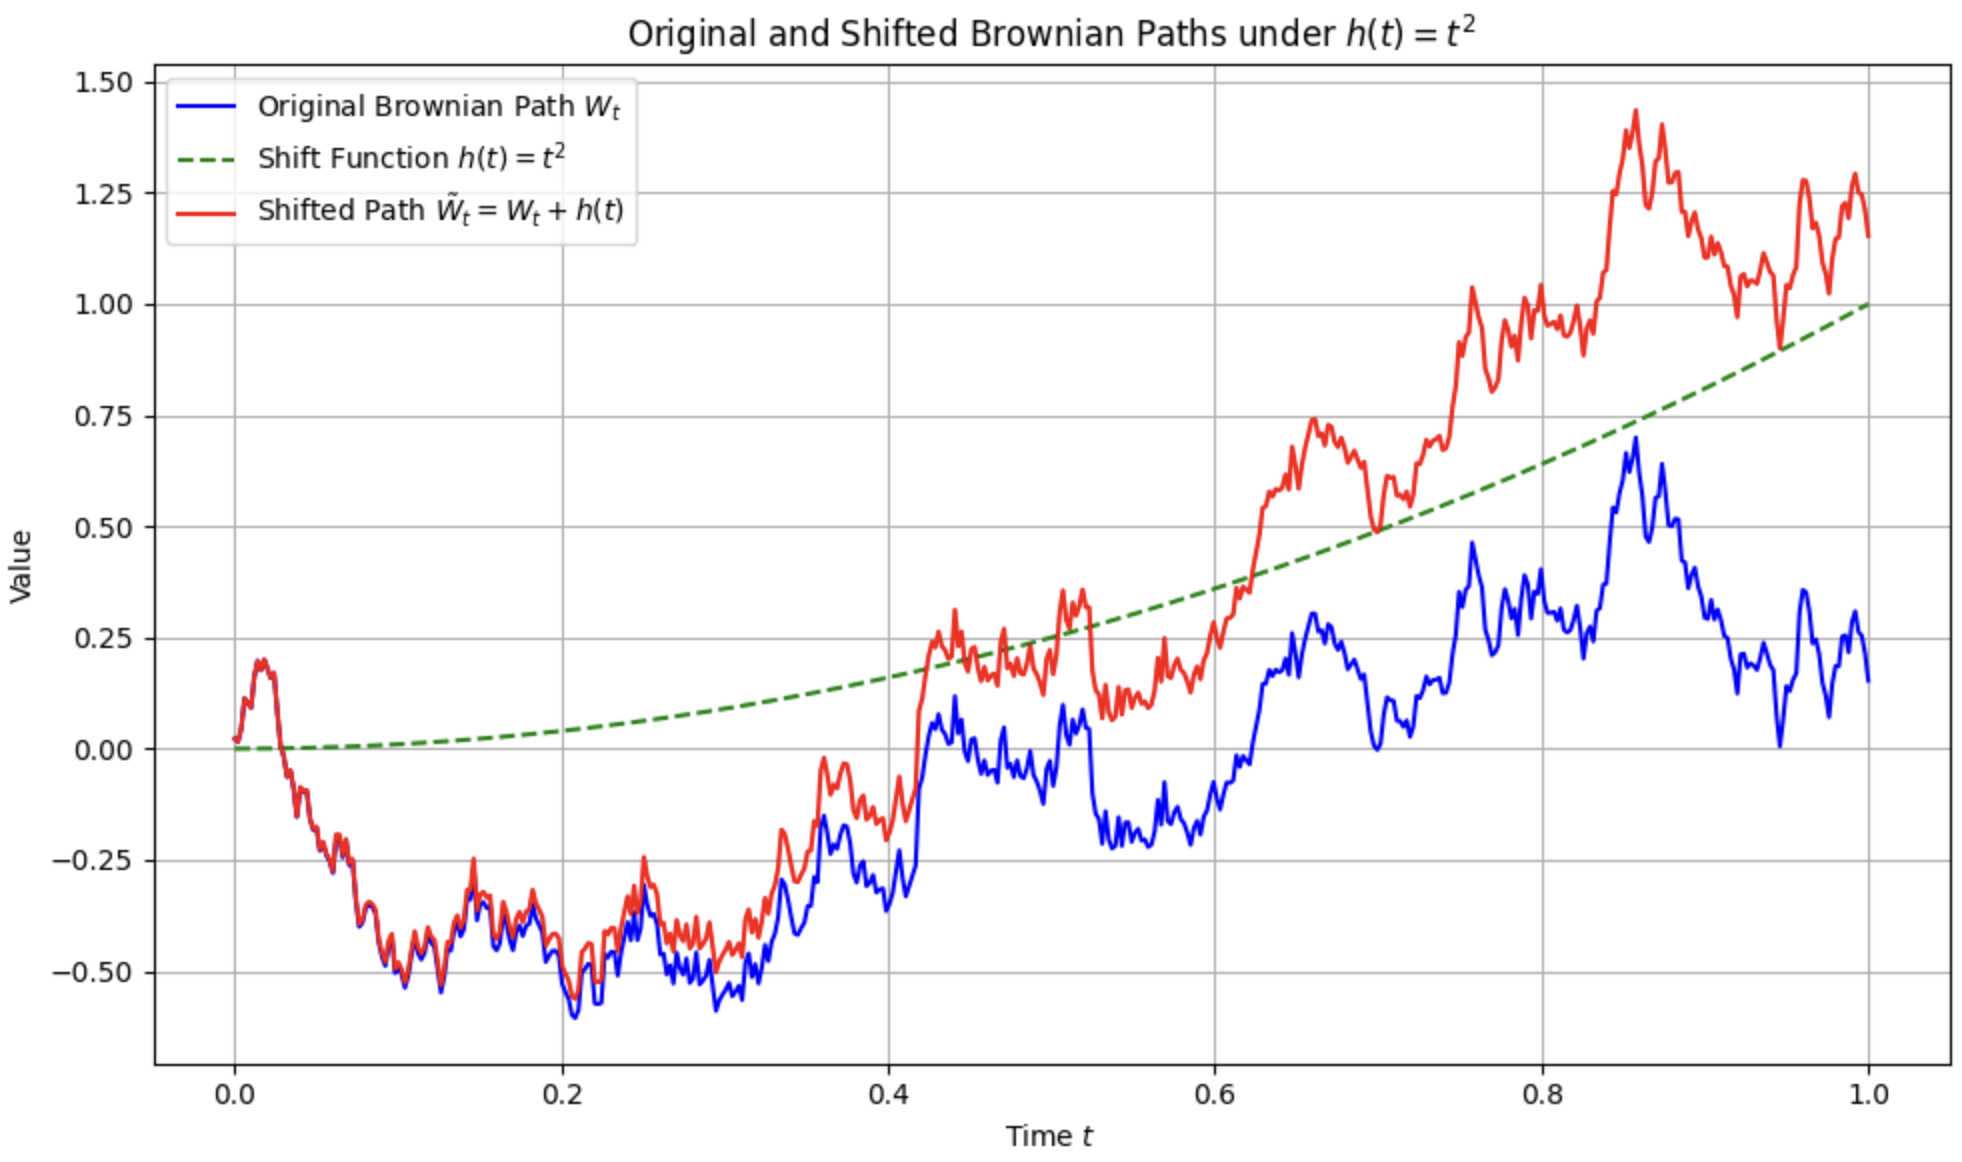
\includegraphics[width=0.8\textwidth]{Shifted Brownian paths.png}
    \caption{Original and shifted paths under \(h(t) = t^2\). The density adjusts via the Radon-Nikodym derivative. \textit{Code: A.4}}
    \label{fig:shift}
\end{figure}

\chapter{Karhunen-Loève Theorem and Spectral Decomposition}
\section{Karhunen-Loève Theorem}
\begin{theorem}[Karhunen-Loève Expansion (1947)] \cite{karatzas}
Let $W= \{W_t\}$, $t \in [a, b] \subset R$; $a, b<1$; be a continuous-parameter real-valued second-order random process with zero
mean and continuous covariance function $K_W(t,\tau)$. Then $\forall \ t\in [a,b]$ decomposition is given as 
\[
W_t = \sum_{k=1}^\infty Z_k \phi_k(t),
\]
with
\[
Z_k = \int_{a}^b W_t\phi_k (t)dt,
\]
where \( \{\phi_k\}_{k=1}^{\infty}\) are eigenfunctions of \(K\) and \(Z_n \sim \mathcal{N}(0, \lambda_n)\).
\end{theorem}
(Description of $\phi_k$: Defining the \textbf{Hilbert-Schmidt integral operator} \(A: L^2([a, b]) \to L^2([a, b])\) by:  
\[
(Af)(t) = \int_a^b K_W(t, \tau) f(\tau) \, d\tau, \quad f \in L^2([a, b]).
\]  
This operator is compact and self-adjoint, guaranteeing a countable set of eigenvalues \(\{\lambda_k\}_{k=1}^\infty\) and corresponding orthonormal eigenfunctions \(\{\phi_k(t)\}_{k=1}^\infty\) that satisfy:  
\[
A e_k = \lambda_k \phi_k, \quad \int_a^b \phi_k(t) \phi_m(t) dt = \delta_{km}.
\]  
The eigenfunctions \(\{\phi_k\}\) form the \textbf{Karhunen-Loève basis} for the subspace spanned by the non-zero eigenvalues of \(A\).
 )

 \begin{proof}
     We will start by defining the Hilbert-Schmidt integral operator $A: L^2[a,b] \rightarrow L^2[a,b]$; where $a,b<1$, defined as
     \[
     (Af)(t) = \int_a^b R(t,s)f(s)ds
     \]
     with $t \in [a,b]$ and $R: [a,b] \times [a,b] \rightarrow R$ assumed continuous in both variables jointly. It is easy to prove that eigen functions of Hilbert-Schmidt operator $A$ corresponding to non zero eigenvalues are continuous on $[a,b]$. We are using a result claiming that if $g: [a,b] \rightarrow \mathbb{R} \text{ is continuous }$ then $g(t)X_t$ is integrable over $[a,b]$.
     Which implies, $Z_k = \int_a^b W_t \phi_k(t)$ is a well defined random variable. Also $E[Z_k]=E[\int_a^bW_t\phi_k(t)]$ and 
     \[
     E[Z_iZ_j] = E[\int_a^b W_t\phi_i(t) dt \int_a^bW_\tau \phi_j(\tau)] = \int_a^b \int_a^b \phi_i(\tau) \phi_j(\tau) \phi_i(t) \phi_j(\tau) K_X(t,\tau) d\tau dt =
     \]
     \[
     \int_a^b \phi_i(\tau) \int_a^b \phi_j(\tau) \phi_i(t) \phi_j(\tau) K_X(t,\tau) d\tau dt = \lambda_i \int_a^b\phi_i(t) \phi_j(t)dt =\lambda_j \delta_{ij}
     \]
     where $\delta_{ij}$ is the Kronecker's delta, by the orthonormality of $\{\phi_k\}_k$ in $L^2[a,b].$ Thus on one hand, since $E[Z_iZ_j]=0,\ \forall i\neq j$, the random variables $\{Z_k\}_{k\in N}$ are pairwise orthogonal in $L^2(\Omega)$, also we know that $\text{Var}(Z_k) := E[Z_kZ_k] = \lambda_k.1 = \lambda_k$.
     Now we need to show the mean square convergence of the series. Let $S_n(t) := \sum_{k=1}^n Z_k\phi_k(t)$. Then 
     \[
     E|S_n(t) - W_t|^2 = E|S_n^2(t)-2S_n(t)X_t+X_t^2| = E[S_n^2(t)]-E[2S_n(t)X_t]+E[X_t^2]
     \]
     Since, $E[X_t]^2 := K_X(t,t)$ and $E[S_n(t)X_t]= E\bigg[\sum_{k=1}^n Z_k\phi_k(t) W_t\bigg] = \sum_{k=1}^n \phi_k(t) E[Z_kW_t]$ and further, $E[S_n^2(t)] = E\bigg[\sum_{i=1}^n Z_i\phi_i(t) \sum_{j=1}^n Z_j \phi_j(t)\bigg] = \sum_{i,j=1}^n \phi_i(t)\phi_j(t)E[Z_iZ_j]$\\
     $=\sum_{i,j=1}^n\phi_i(t)\phi_j(t)\lambda_{ij}\delta_{ij}=\sum_{k=1}^n \lambda_k\phi_k^2(t)$. Putting all together,
     \[
     E|S_n(t) -W_t|^2 = \sum_{k=1}^n \lambda_k\phi_k^2(t)- 2\sum_{i=1}^n\phi_k(t) E[Z_kW_t]  +K _X(t,t).
     \]
     Now, we will use an important result which states that if $h:[a,b] \rightarrow \mathbb{R}$ and $K_x: [a,b]\times [a,b] \rightarrow \mathbb{R}$ are continuous, then for every $t\in [a,b]$
     \[
     E\bigg[W_t\int_a^bh(\tau)W_\tau d\tau \bigg] = \int_a^bh(\tau)K_W(t,\tau) d\tau.
     \]
     Using this result, $E[Z_kW_t] = E[W_t \int_a^bW_\tau \phi_k(\tau)d\tau = \int_a^b \phi_k(\tau) K_W(t,\tau)d\tau =\lambda_k\phi_k(t)$. Thus,
     \begin{align*}
         E|S_n(t) - W_t|^2 &= \sum_{k=1}^n\lambda_k\phi_k^2(t) - 2\sum_{k=1}^n \lambda_k\phi_k^2(t) + K_W(t,t) \\
         &= K_W(t,t) - \sum_{k=1}^n\lambda_k\phi_k^2(t)\\
         & \xrightarrow{n\rightarrow\infty} 0 ,
     \end{align*}
     uniformly in $t\in [a,b]$ by Mercer's Theorem.
 \end{proof}

\subsection{Covariance Eigenanalysis}  
The covariance structure of Brownian motion is encoded in its kernel \(K(t, s) = \min(t, s)\). To derive the eigenfunctions \(\phi_n(t)\) and eigenvalues \(\lambda_n\) of the associated Hilbert-Schmidt operator, we solve the integral equation \cite{karatzas}:  
\[
\int_0^1 \min(t, s) \phi(s) \, ds = \lambda \phi(t), \quad t \in [0, 1].
\]
This subsection details the solution to this equation, yielding the spectral decomposition of Brownian motion.

\subsubsection{Splitting the Integral}  
Using the piecewise definition of \(\min(t, s)\), the integral splits into two regions:  
\[
\int_0^t s \phi(s) \, ds + \int_t^1 t \phi(s) \, ds = \lambda \phi(t).
\]
Differentiate both sides with respect to \(t\) to simplify. Applying Leibniz’s rule:  
\[
\frac{d}{dt} \left[\int_0^t s \phi(s) \, ds\right] = t \phi(t), \quad \frac{d}{dt} \left[t \int_t^1 \phi(s) \, ds\right] = \int_t^1 \phi(s) \, ds - t \phi(t).
\]
Combining these, the derivative of the left-hand side becomes:  
\[
t \phi(t) + \int_t^1 \phi(s) \, ds - t \phi(t) = \int_t^1 \phi(s) \, ds.
\]
The derivative of the right-hand side is \(\lambda \phi'(t)\). Thus:  
\[
\int_t^1 \phi(s) \, ds = \lambda \phi'(t).
\]

\subsubsection{Second Differentiation}  
Differentiate again with respect to \(t\):  
\[
-\phi(t) = \lambda \phi''(t).
\]
Rearranging gives the ordinary differential equation (ODE):  
\[
\phi''(t) + \frac{1}{\lambda} \phi(t) = 0.
\]
This is the harmonic oscillator equation, with general solution:  
\[
\phi(t) = A \sin\left(\frac{t}{\sqrt{\lambda}}\right) + B \cos\left(\frac{t}{\sqrt{\lambda}}\right).
\]

\subsubsection{Boundary Conditions}  
From the original integral equation:  
\begin{enumerate}[label=(\roman*)]
    \item At \(t = 0\): \(\int_0^1 0 \cdot \phi(s) \, ds = \lambda \phi(0) \implies \phi(0) = 0\).  
    \item At \(t = 1\): \(\int_0^1 s \phi(s) \, ds = \lambda \phi(1)\).  
\end{enumerate}
From \(\phi(0) = 0\), we find \(B = 0\), so \(\phi(t) = A \sin\left(\frac{t}{\sqrt{\lambda}}\right)\).  

Using the first derivative condition from earlier, \(\int_t^1 \phi(s) \, ds = \lambda \phi'(t)\). At \(t = 1\):  
\[
0 = \lambda \phi'(1) \implies \phi'(1) = 0.
\]
Differentiating \(\phi(t)\):  
\[
\phi'(t) = \frac{A}{\sqrt{\lambda}} \cos\left(\frac{t}{\sqrt{\lambda}}\right).
\]
Setting \(t = 1\):  
\[
\cos\left(\frac{1}{\sqrt{\lambda}}\right) = 0 \implies \frac{1}{\sqrt{\lambda}} = \frac{(2n - 1)\pi}{2}, \quad n \in \mathbb{N}.
\]
Thus, the eigenvalues are:  
\[
\lambda_n = \left(\frac{2}{(2n - 1)\pi}\right)^2.
\]

\subsubsection{Eigenfunction Normalization}  
The eigenfunctions are \(\phi_n(t) = A \sin\left(\frac{(2n - 1)\pi t}{2}\right)\). To normalize \(\|\phi_n\|_{L^2} = 1\):  
\[
\int_0^1 \phi_n^2(t) \, dt = A^2 \int_0^1 \sin^2\left(\frac{(2n - 1)\pi t}{2}\right) dt = \frac{A^2}{2} \implies A = \sqrt{2}.
\]
Thus, the orthonormal eigenfunctions are:  
\[
\phi_n(t) = \sqrt{2} \sin\left(\frac{(2n - 1)\pi t}{2}\right), \quad n = 1, 2, \dots
\]

\paragraph*{Conclusion}  
The eigenfunctions \(\phi_n(t)\) and eigenvalues \(\lambda_n\) diagonalize the covariance operator of Brownian motion, forming the basis for its Karhunen-Loève decomposition.  

\section{Example: Numerical Simulation}
\begin{example}[Truncated Karhunen-Loève Expansion]
Approximating \(W_t\) using \(N=200\) terms:
\[
W_t^{(N)} = \sum_{n=1}^{200} Z_n \sqrt{\lambda_n} \phi_n(t).
\]
Figure \ref{fig:kl} compares the approximation to a simulated path.
\end{example}
This approximation represents $W_t$ as a finite sum of smooth sine functions. It shows the essential statistical properties of $W_t$ in $L^2$-sense (mean-square convergence).\\
\\
Steps to generate $W_t^{200}$ follows generating random coefficients from sample $Z_n\sim\mathcal{N}(0,1)$ for $n=1,2,... 200$, then computing eigen values and eigen functions $\sqrt{\lambda_n}\phi_n(t) = \frac{2\sqrt{2}}{(2n-1)\pi}\sin\bigg(\frac{(2n-1)\pi t}{2}\bigg).$

\begin{figure}[H]
    \centering
    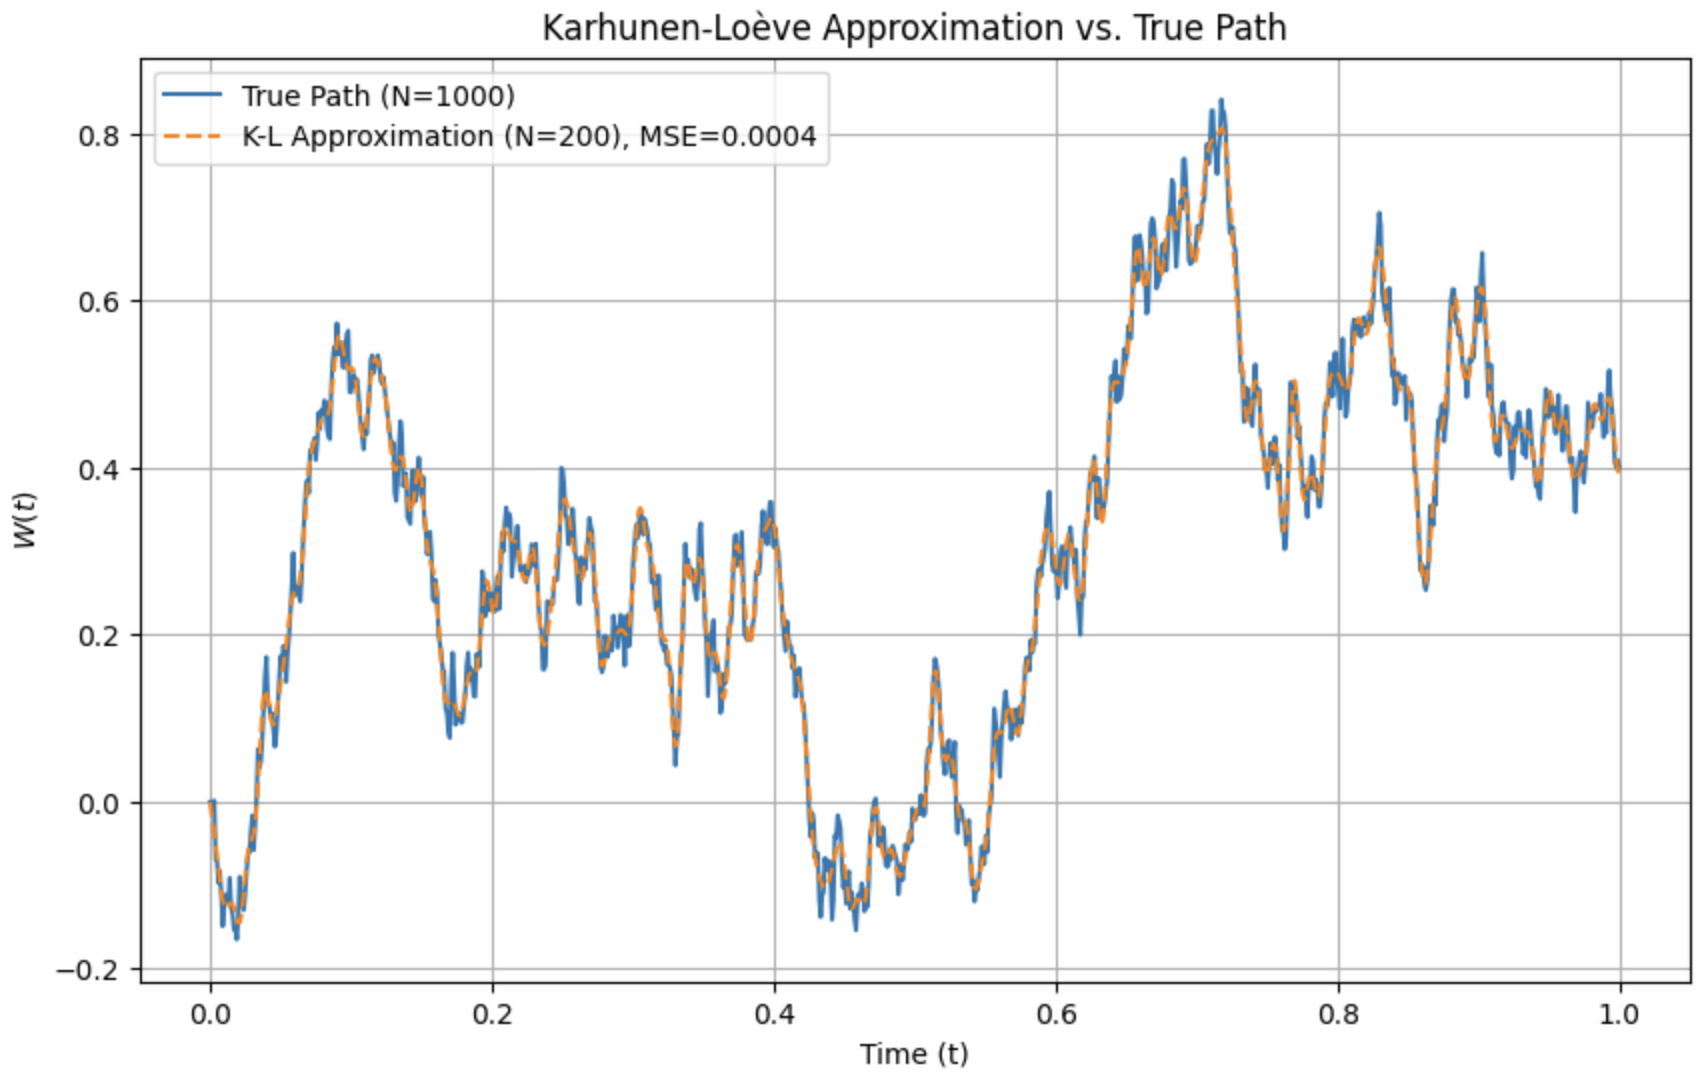
\includegraphics[width=0.8\textwidth]{K-L approximation.png}
    \caption{Karhunen-Loève approximation vs True path, For K-L approximation, each term $Z_n\sqrt{\lambda_n}\phi_n(t)$ is computed and summed to build the approximation of the Wiener process. \textit{Code: A.5}}
    \label{fig:kl}
\end{figure}

\chapter{Applications and Interdisciplinary Connections}

Brownian motion is used as one of the primary and fundamental tool in modern probability theory, having deep uses across mathematical analysis, physics, finance, and engineering. In this chapter, we will try to describe two key application areas, stochastic calculus and financial mathematics.

\section{Stochastic Calculus}

The theory of stochastic calculus is fundamentally built upon the probabilistic structure of Brownian motion. The Itô integral
\[
\int_0^T f(t) \, dW_t,
\]
is defined for suitable adapted processes \( f \) and exploits the martingale and quadratic variation properties of Brownian paths. The Itô isometry and Itô’s lemma form the basis for solving stochastic differential equations (SDEs), which model systems influenced by random noise.

\section{Financial Mathematics}

In quantitative finance, Brownian motion models the unpredictable dynamics of asset prices. The Black–Scholes model asserts that the price \( S_t \) of a risky asset evolves according to the geometric Brownian motion:
\[
dS_t = \mu S_t \, dt + \sigma S_t \, dW_t,
\]
where \( \mu \in \mathbb{R} \) is the drift rate and \( \sigma > 0 \) is the volatility.

A central concept which is used primarily in pricing theory is the change of measure from the real-world probability measure \( \mathbb{P} \) to a risk-neutral measure \( \mathbb{Q} \). For this measure discounted asset prices become martingales. This transformation involves modifying the drift of the Brownian motion, leading to a new process:
\[
dW_t^\mathbb{Q} = dW_t + \theta_t \, dt,
\]
where \( \theta_t \) represents the market price of risk.



\chapter{Conclusion}

In this project, we have shown how the functional analytic framework is utilised to understand Brownian motion by looking at three essential tools in infinite-dimensional stochastic analysis. We started with Wiener's construction, which included illustrative Python code as well as the Fourier series representation and the finite-dimensional approximations of Brownian paths. This illustrated how abstract Wiener space provides a rigorous measure-theoretic foundation for modeling Brownian motion.\\
\\
\noindent
We then looked at the Cameron–Martin theorem, which explains how deterministic shifts of Brownian paths change the Wiener measure. Although we only provided a basic overview of the proof, we discussed its key implications and demonstrated how deterministic shifts impact things through simulation.\\
\\
\noindent
Finally, we looked at the Karhunen–Loeve theorem, discussing its spectral decomposition of Brownian motion and providing a comprehensive demonstration. In practical contexts, this decomposition not only demonstrates the orthogonal structure of Gaussian processes but also acts as a link to dimension reduction methods.\\
\\
\noindent
In order to improve intuition and highlight important phenomena, we added Python simulations to our theoretical presentation throughout the report. These elements work together to create a coherent image of the theoretical and practical interactions between stochastic processes and functional analysis.


\appendix
\chapter{Computational Appendix}
\section{Simulating Brownian Motion}
\begin{verbatim}
import numpy as np
import matplotlib.pyplot as plt

def brownian_motion(T=1, N=1000):
    dt = T/N
    dW = np.random.normal(0, np.sqrt(dt), N)
    W = np.cumsum(dW)
    return W

t = np.linspace(0, 1, 1000)
W = brownian_motion()
plt.plot(t, W)
\end{verbatim}

\section{Symmetric and Scaled Random Walk}
\begin{verbatim}
import numpy as np
import matplotlib.pyplot as plt

def symmetric_random_walk(n_steps):
    # Generating steps: 50% chance of +1, 50% chance of -1
    steps = np.random.choice([-1, 1], size=n_steps)
    # Computing cumulative sum starting at 0
    walk = np.cumsum(steps)
    return np.concatenate(([0], walk))

def scaled_random_walk(n_steps, T=1):
    dt = T / n_steps
    scaling_factor = np.sqrt(dt)
    # Generating steps and scale them
    steps = np.random.choice([-1, 1], size=n_steps) * scaling_factor
    # Computing cumulative sum starting at 0
    walk = np.cumsum(steps)
    return np.concatenate(([0], walk))

# Example
n_steps = 1000  # Number of steps
T = 1           # Total time for the scaled walk

# Generating walks
walk_sym = symmetric_random_walk(n_steps)
walk_scaled = scaled_random_walk(n_steps, T)

# Creating time arrays for plotting
time_steps_sym = np.arange(n_steps + 1)  
time_scaled = np.linspace(0, T, n_steps + 1)  

# Plotting
plt.figure(figsize=(12, 6))

# Symmetric Random Walk
plt.subplot(1, 2, 1)
plt.plot(time_steps_sym, walk_sym)
plt.title("Symmetric Random Walk")
plt.xlabel("Step")
plt.ylabel("Position")

# Scaled Random Walk
plt.subplot(1, 2, 2)
plt.plot(time_scaled, walk_scaled)
plt.title("Scaled Random Walk (Time Scaled)")
plt.xlabel("Time")
plt.ylabel("Position")

plt.tight_layout()
plt.show()
\end{verbatim}

\section{Quadratic variation convergence}
\begin{verbatim}
import numpy as np
import matplotlib.pyplot as plt

# Parameters
n = 10**4
T = 1.0
dt = T / n

# Brownian motion
np.random.seed(42)
dW = np.sqrt(dt) * np.random.randn(n)
W = np.cumsum(dW)

# Quadratic variation as the sum of squared increments
quad_var = np.cumsum(dW**2)

# Time axis
t = np.linspace(dt, T, n)

# Plotting
plt.figure(figsize=(10, 6))
plt.plot(t, quad_var, label='Quadratic Variation of $W_t$', color='blue')
plt.plot(t, t, '--', label='t (Reference Line)', color='red')
plt.xlabel('Time')
plt.ylabel('Quadratic Variation')
plt.title('Quadratic Variation Convergence for Brownian Motion ($n=10^4$)')
plt.legend()
plt.grid(True)
plt.tight_layout()
plt.show()
\end{verbatim}

\section{Shifted Brownian Motion}
\begin{verbatim}
import numpy as np
import matplotlib.pyplot as plt
np.random.seed(42)

# Time discretization
T = 1.0
N = 500
t = np.linspace(0, T, N)
dt = t[1] - t[0]

# Brownian motion path
W = np.cumsum(np.sqrt(dt) * np.random.randn(N))

# Deterministic shift h(t) = t^2
h = t**2

# Shifted Brownian motion
W_tilde = W + h

# Plotting
plt.figure(figsize=(10, 6))
plt.plot(t, W, label="Original Brownian Path $W_t$", color='blue')
plt.plot(t, h, label="Shift Function $h(t) = t^2$", color='green', linestyle='--')
plt.plot(t, W_tilde, label="Shifted Path $\\tilde{W}_t = W_t + h(t)$", color='red')
plt.xlabel("Time $t$")
plt.ylabel("Value")
plt.title("Original and Shifted Brownian Paths under $h(t) = t^2$")
plt.legend()
plt.grid(True)
plt.tight_layout()
plt.show()
\end{verbatim}

\section{Karhunen-Loève Implementation}
\begin{verbatim}
import numpy as np
import matplotlib.pyplot as plt

# Parameters
np.random.seed(42) 
N_true = 1000       
N_approx = 200      
M = 1000           
t = np.linspace(0, 1, M)
Z = np.random.normal(size=N_true)

# Initializing paths
W_true = np.zeros_like(t)    
W_approx = np.zeros_like(t)  # K-L approximation (N_approx terms)

# Computing the K-L expansions
for n in range(1, N_true + 1):
    # Eigenvalue and eigenfunction for the nth term
    coefficient = (2 * np.sqrt(2)) / ((2 * n - 1) * np.pi)
    sin_term = np.sin((2 * n - 1) * np.pi * t / 2)
    # Add to the true path
    W_true += Z[n-1] * coefficient * sin_term
    # Add to the approximation if n <= N_approx
    if n <= N_approx:
        W_approx += Z[n-1] * coefficient * sin_term

# Computing MSE
mse = np.mean((W_true - W_approx)**2)

# Plotting
plt.figure(figsize=(10, 6))
plt.plot(t, W_true, label=f'True Path (N={N_true})', linewidth=1.5)
plt.plot(t, W_approx, '--', label=f'K-L Approximation (N={N_approx}), MSE={mse:.4f}', linewidth=1.5)
plt.title('Karhunen-Loève Approximation vs. True Path')
plt.xlabel('Time (t)')
plt.ylabel('$W(t)$')
plt.legend()
plt.grid(True)
plt.show()
\end{verbatim}

\begin{thebibliography}{9}
\bibitem{conway} 
Conway, J. B. (1990). \textit{A Course in Functional Analysis}. Springer.

\bibitem{bobrowski} 
Bobrowski, A. (2005). \textit{Functional Analysis for Probability and Stochastic Processes}. Cambridge University Press.

\bibitem{karatzas} 
Karatzas, I., \& Shreve, S. E. (1991). \textit{Brownian Motion and Stochastic Calculus}. Springer.

\bibitem{cameron} 
Cameron, R. H., \& Martin, W. T. (1944). Transformations of Wiener Integrals. \textit{Transactions of the AMS}.
\end{thebibliography}

\end{document}